\documentclass[11pt]{article}

% This first part of the file is called the PREAMBLE. It includes
% customizations and command definitions. The preamble is everything
% between \documentclass and \begin{document}.

\usepackage[margin=1in]{geometry}  % set the margins to 1in on all sides
\usepackage{graphicx}              % to include figures
\usepackage{amsmath}               % great math stuff
\usepackage{amsfonts}              % for blackboard bold, etc
\usepackage{amsthm}                % better theorem environments

\usepackage{array}
\usepackage{booktabs}
\usepackage{soul}
\usepackage{mathrsfs}
\usepackage{enumerate}
\usepackage{multicol}
\usepackage[makeroom]{cancel}
\usepackage{xcolor}
\usepackage{tikz}
\usepackage{pdfpages}

% various theorems, numbered by section

\newtheorem{thm}{Theorem}[section]
\newtheorem{lem}[thm]{Lemma}
\newtheorem{prop}[thm]{Proposition}
\newtheorem{cor}[thm]{Corollary}
\newtheorem{conj}[thm]{Conjecture}
\newtheorem{exer}[thm]{Exercise}

\DeclareMathOperator{\id}{id}

\newcommand{\bd}[1]{\mathbf{#1}}  % for bolding symbols
\newcommand{\RR}{\mathbb{R}}      % for Real numbers
\newcommand{\ZZ}{\mathbb{Z}}      % for Integers
\newcommand{\col}[1]{\left[\begin{matrix} #1 \end{matrix} \right]}
\newcommand{\comb}[2]{\binom{#1^2 + #2^2}{#1+#2}}
\newcommand{\overfrac}[2]{\genfrac{}{}{0pt}{}{#1}{#2}}

\renewcommand{\thesubsection}{\thesection.\alph{subsection}}

\everymath{\displaystyle}

\setlength\parindent{0pt}

\usepackage{setspace}

\begin{document}
\begin{multicols}{2}
  \phantom{hello}\vspace{\baselineskip}
  \phantom{hello}\vspace{\baselineskip}
  {\large Assignment 3}\\
  \begin{flushright}
    Mikhail Gaerlan (914437675)\\
    21 April 2017\\
    STA 243 Lee
  \end{flushright}
\end{multicols}
\vspace{-1.3\baselineskip}

\hrulefill

\section{}

\subsection{}
\begin{eqnarray*}
  \ell(\theta)&=&x_1\log\left(2+\theta\right)+\left(x_2+x_3\right)\log\left(1-\theta\right)+x_4\log\theta+c\\
              &=&125\log\left(2+\theta\right)+\left(18+19\right)\log\left(1-\theta\right)+35\log\theta+c\\
  \ell'(\theta)&=&\frac{125}{2+\theta}+\frac{37}{1-\theta }+\frac{35}{\theta }\\
              &=&\frac{-197 \theta ^2+16 \theta +70}{(\theta +2)(1-\theta) \theta }
\end{eqnarray*}
Thus the MLE is found by setting the numerator of the derivative of the log-likelihood to zero.
\begin{eqnarray*}
  0&=&-197 \theta ^2+16 \theta +70\\
  \theta&=&\frac{1}{197} \left(8\pm\sqrt{13854}\right)\\
   &\approx&-0.556868,0.638086
\end{eqnarray*}
Since $0\leq\theta\leq1$, then the MLE is $\theta=\frac{1}{197} \left(8+\sqrt{13854}\right)\approx0.638086$.

\subsection{}

\underline{E-Step:} Calculate
\begin{eqnarray*}
  Q(\theta\,|\,\theta^{\left(k\right)})&=&\mathbb{E}_{\theta^{\left(k\right)}}\left\{\ell_c\left(\theta\right)|\,y\right\}\\
                                                  &=&\mathbb{E}_{\theta^{\left(k\right)}}\left\{\left(x_{12}+x_4\right)\log\theta+\left(x_2+x_3\right)\log\left(1-\theta\right)|\,y\right\}\\
                                                  &=&\mathbb{E}_{\theta^{\left(k\right)}}\left\{x_{12}\,|\,y\right\}\log\theta+x_4\log\theta+\left(x_2+x_3\right)\log\left(1-\theta\right)\\
                                                  &=&\frac{\theta^{\left(k\right)}\left(1+x_2+x_3+x_4\right)!}{\left(1-\theta^{\left(k\right)}\right)^2\left(x_2+x_3+x_4\right)!}\log\theta+x_4\log\theta+\left(x_2+x_3\right)\log\left(1-\theta\right)\\
\end{eqnarray*}

\underline{M-Step:} Maximize $Q(\theta\,|\,\theta^{\left(k\right)})$ with respect to $\theta$.
\begin{eqnarray*}
  \frac{dQ(\theta^{\left(k+1\right)},|\,\theta^{\left(k\right)})}{d\theta}&=&0\\
                                                                                     &=&\frac{1}{\theta^{\left(k+1\right)}}\frac{\theta^{\left(k\right)}}{\left(1-\theta^{\left(k\right)}\right)^2}\frac{\left(1+x_2+x_3+x_4\right)!}{\left(x_2+x_3+x_4\right)!}+\frac{x_4}{\theta^{\left(k+1\right)}}-\frac{x_2+x_3}{1-\theta^{\left(k+1\right)}}\\
  \theta^{\left(k+1\right)}&=&\frac{\theta^{\left(k\right)}\left(1+x_2+x_3+x_4\right)!+x_4\left(1-\theta^{\left(k\right)}\right)^2\left(x_2+x_3+x_4\right)!}{\theta^{\left(k\right)}\left(1+x_2+x_3+x_4\right)!+\left(x_2+x_3+x_4\right)\left(1-\theta^{\left(k\right)}\right)^2\left(x_2+x_3+x_4\right)!}
\end{eqnarray*}

\subsection{}

I don't know actually how to calculate $Q\dots$ so $\theta^{\left(k\right)}\rightarrow1$ as $k\rightarrow\infty$ which is not right$\dots$

\section{}

\subsection{}

First, find the CDF of the Weibull distribution,
\begin{eqnarray*}
  w\left(x\,|\,\alpha\right)&=&\int_0^xW\left(t\,|\,\alpha\right)dt\\
                            &=&\int_0^x\frac{2t}{\alpha^2}e^{-\frac{t^2}{\alpha^2}}dt\\
                            &=&\left.-e^{-\frac{t^2}{\alpha^2}}\right|_0^x\\
                            &=&1-e^{-\frac{x^2}{\alpha^2}}
\end{eqnarray*}

Then, find the complete log-likelihood function
\begin{eqnarray*}
  \ell_c\left(\alpha\right)&=&\sum_u\log\left(W\left(x_i\,|\,\alpha\right)\right)+\sum_c\log\left(1-w\left(x_i\,|\,\alpha\right)\right)\\
                           &=&\sum_u\log\left(\frac{2x_i}{\alpha^2}e^{-\frac{x_i}{\alpha^2}}\right)+\sum_c\log\left(e^{-\frac{x_i^2}{\alpha^2}}\right)\\
                           &=&\sum_u\log\left(\frac{2x_i}{\alpha^2}\right)-\sum_{i=1}^n\frac{x_i^2}{\alpha^2}
\end{eqnarray*}

Then, the E-step is
\begin{eqnarray*}
  Q(\alpha\,|\,\alpha^{\left(k\right)})&=&\mathbb{E}_{\alpha^{\left(k\right)}}\left\{\ell_c\left(\theta\right)|\,y\right\}
\end{eqnarray*}
and the M-step is
\begin{eqnarray*}
  \frac{dQ(\alpha^{\left(k+1\right)},|\,\alpha^{\left(k\right)})}{d\alpha}&=&0
\end{eqnarray*}

\subsection{}

\section{}

\begin{align*}
  f(x)&=c\,e^{-x},\qquad 0<x<2\\
  c^{-1}&=\int_0^2e^{-x}dx&  F(x)&=\frac{\displaystyle \int_0^xe^{-t}dt}{1-e^{-2}}\\
      &=\left.-e^{-x}\right\rvert_0^2&      &=\frac{1-e^{-x}}{ 1-e^{-2}}\\
      &=1-e^{-2}
\end{align*}
First sample $u$ from $\textrm{unif}(0,1)$, then find $F^{-1}(u)$. Equivalently solve $F(x)-u=0$.
\begin{eqnarray*}
  0&=&F(x)-u\\
  0&=&\frac{1-e^{-x}}{ 1-e^{-2}}-u\\
  0&=&1-e^{-x}-\left(1-e^{-2}\right)u\\
  x&=&-\log\left(1-\left(1-e^{-2}\right)u\right)
\end{eqnarray*}

The results are displayed in Figure \ref{inverse}. The gray bars represent frequency. The white bars represent the cumulative frequency. The lines represent the estimated densities.

\begin{figure}[h!]
  \begin{center}
    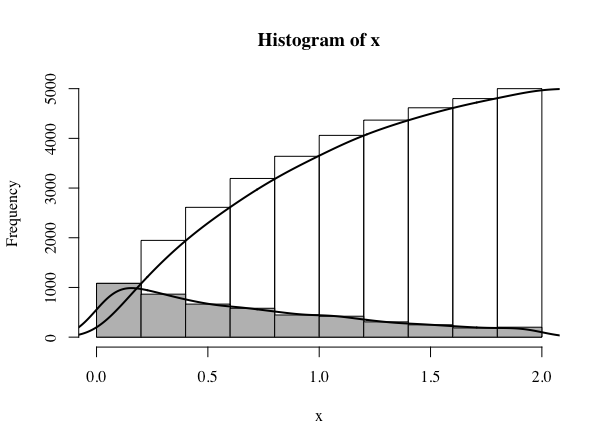
\includegraphics[height=0.32\textheight,width=0.6\linewidth]{inversetransform}
  \end{center}
  \caption{\textbf{Problem 3.}}
  \label{inverse}
\end{figure}

\section{}

\subsection{}

\begin{eqnarray*}
  \alpha_1&=&\sup_{0<x}\frac{q(x)}{g_1(x)}=\sup_{0<x}\frac{\displaystyle \frac{e^{-x}}{1+x^2}}{e^{-x}}=\sup_{x>0}\frac{1}{1+x^2}=1\\
  \alpha_2&=&\sup_{0<x}\frac{q(x)}{g_2(x)}=\sup_{0<x}\frac{\displaystyle \frac{e^{-x}}{1+x^2}}{\displaystyle \frac{2}{\pi\left(1+x^2\right)}}=\sup_{x>0}\frac{\pi}{2}e^{-x}=\frac{\pi}{2}
\end{eqnarray*}

Use the inverse transform to sample $x$ from $g_1(x)$ and $g_2(x)$ using $u$ from $\textrm{unif}(0,1)$.
\begin{align*}
  G_1(x)&=\int_0^xe^{-t}dt&G_2(x)&=\frac{2}{\pi}\int_0^x\frac{1}{1+t^2}dt\\
        &=1-e^{-x}& &=\frac{2}{\pi}\tan^{-1}x\\
  x&=-\log(1-u)&x&=\tan\left(\frac{\pi}{2}u\right)
\end{align*}

The results are shown in Table \ref{double}.

\begin{table}[h!]
  \begin{center}
    \renewcommand{\arraystretch}{1.5}
    \begin{tabular}{|c|c|}
      \hline
      Sampling $f(x)$ using $g_1(x)$&Sampling $f(x)$ from $g_2(x)$\\\hline
      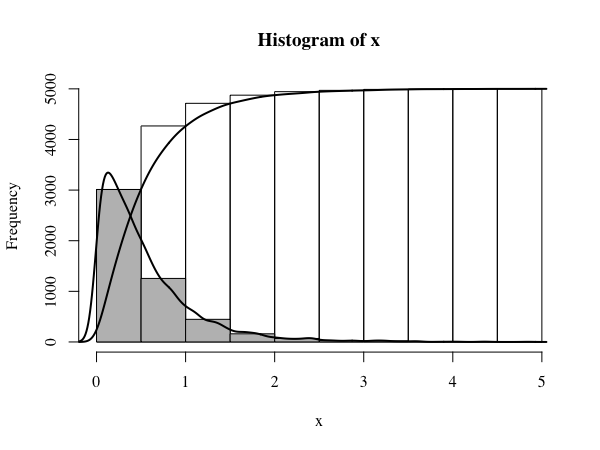
\includegraphics[width=0.42\linewidth,height=0.23\textheight]{density4a1}&
      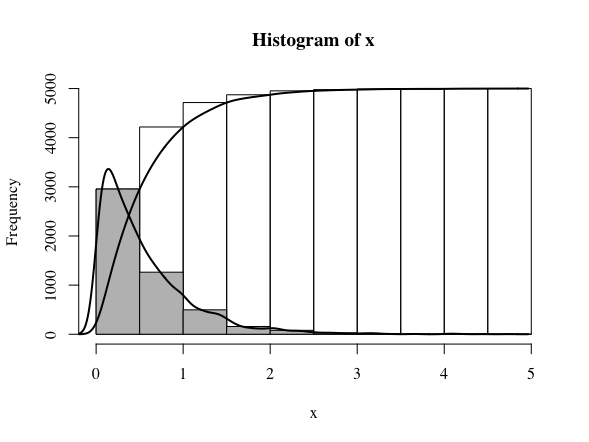
\includegraphics[width=0.42\linewidth,height=0.23\textheight]{density4a2}\\\hline
    \end{tabular}
  \end{center}
  \caption{\textbf{Problem 4.}}
  \label{double}
\end{table}

\subsection{}

The number of iterations needed to produce 5,000 data points required approximately 8,000 iterations using $g_1(x)$ and 11,000 iterations using $g_2(x)$. This makes sense since the $\alpha_1<\alpha_2$ and the acceptance probability, which is inversely proportional to the $\alpha$ value, is higher for $g_1(x)$.

\section{}

First, the problem can be converted into polar coordinates with the form 
\begin{equation*}
  f\left(r,\theta\right)\propto r^\alpha\cos^\alpha\theta\,r\sin\theta=r^{\alpha+1}\cos^\alpha\theta\sin\theta=q\left(r,\theta\right),\quad 0<r\leq1,\quad 0<\theta<\frac{\pi}{2}
\end{equation*}
where $\alpha>-1$ since otherwise $f(r,\theta)$ would not be a probability distribution since the integral would not converge over the domain for $\alpha\leq-1$. $f(r,\theta)$ is now easily integrable where $f(r,\theta) = c\,q\left(r,\theta\right)$ and
\begin{eqnarray*}
  c^{-1}&=&\int_0^{\frac{\pi}{2}}\int_0^1r^{\alpha+1}\cos^\alpha\theta\sin\theta\,r\,dr\,d\theta\\
        &=&\frac{1}{\alpha+3}\left.r^{\alpha+3}\right\rvert_0^1\frac{1}{\alpha+1}\left.\cos^{\alpha+1}\theta\right\rvert_0^\frac{\pi}{2}\\
        &=&\frac{1}{\alpha+3}\frac{1}{\alpha+1}\\
  c&=&\left(\alpha+3\right)\left(\alpha+1\right)>1,\quad\alpha>-1
\end{eqnarray*}
Then sample $\left(x,y\right)$ from $\left[\,0,1\,\right]\times\left[\,0,1\,\right]$. If $x^2+y^2\leq1$, then accept $\left(x,y\right)$. Now sample $u$ uniformly from $\left[\,0,1\,\right]$ and accept $\left(x,y\right)$ if $u \leq f(x,y)/\left(\beta\,g\left(x,y\right)\right)$ where $\beta=\sup_{(x,y)\in\mathbb{R}^2}f(x,y)/g(x,y)$ and $f(x,y)\leq c\,g(x,y)$ for all $(x,y)$ in the upper right quarter of the unit disc and $c>0$

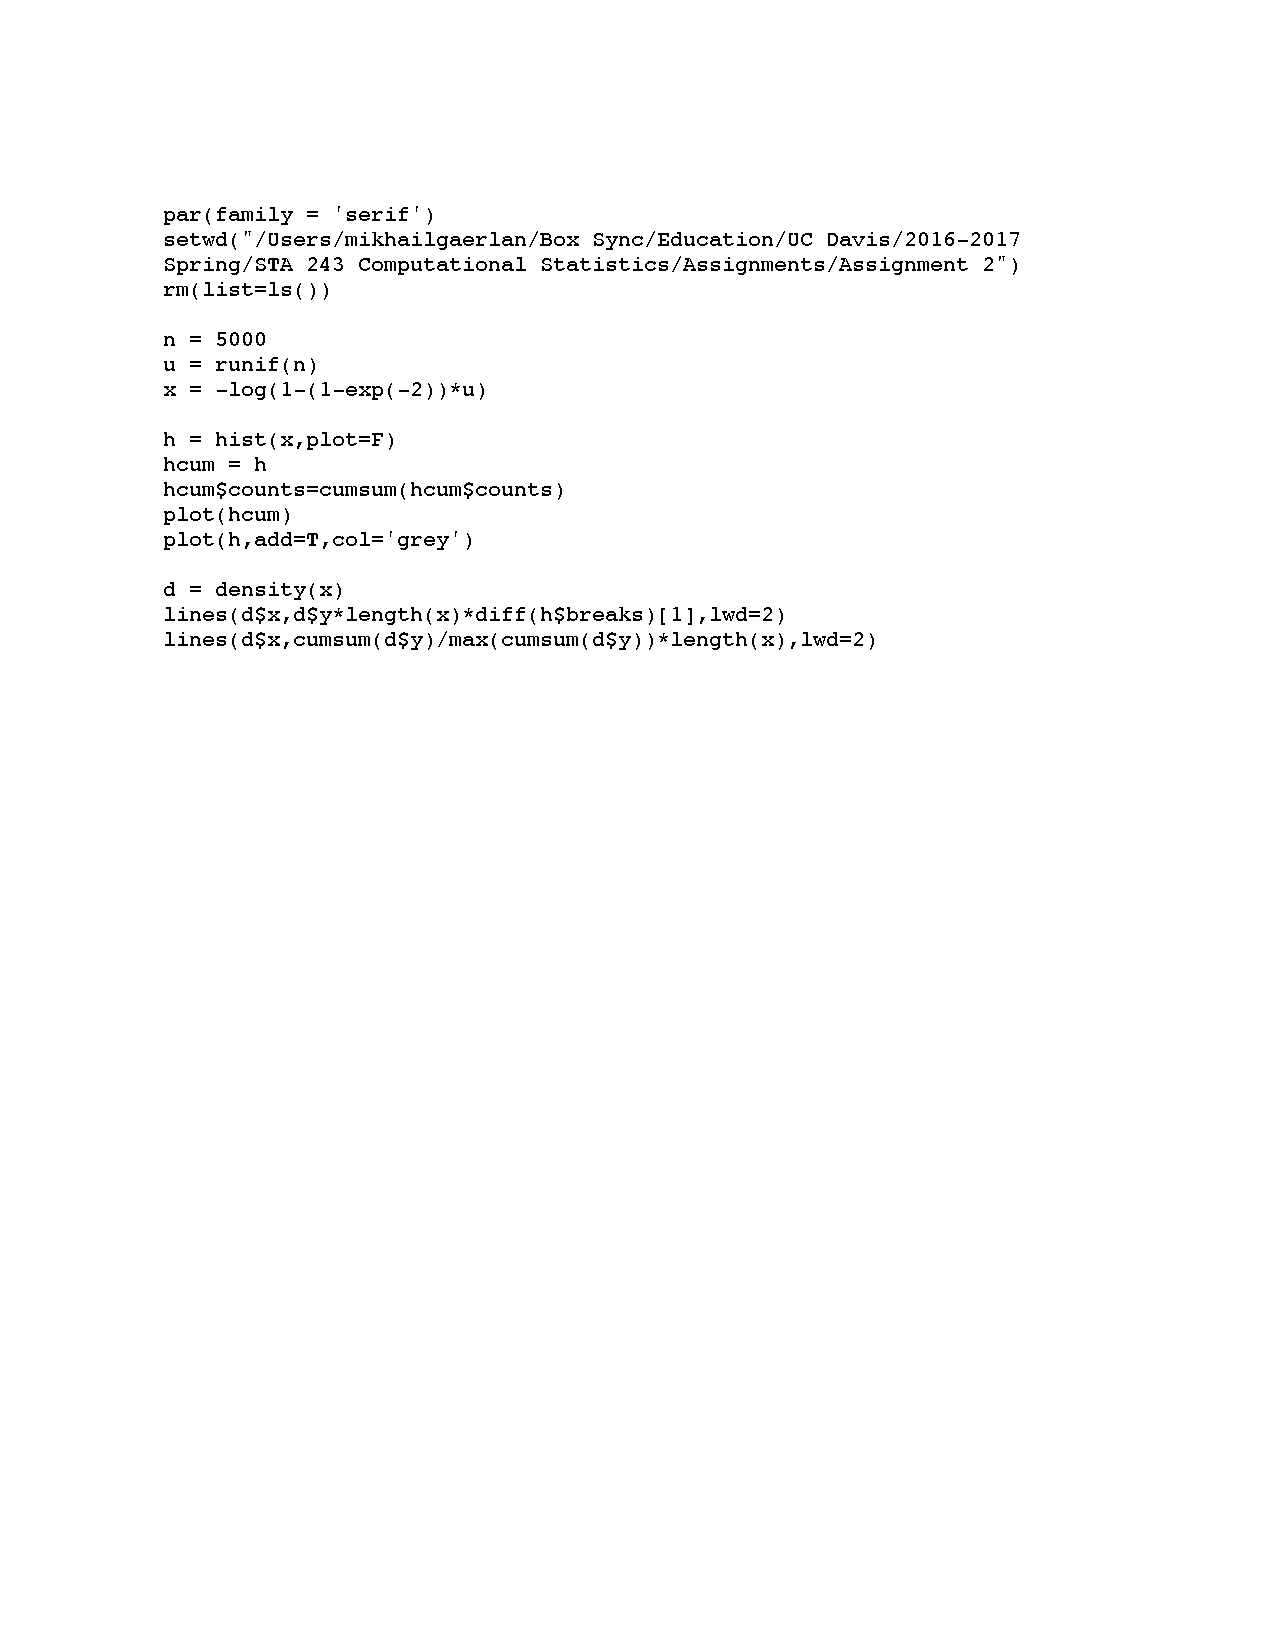
\includepdf[pages={1-1}]{Code/assignment31.pdf}
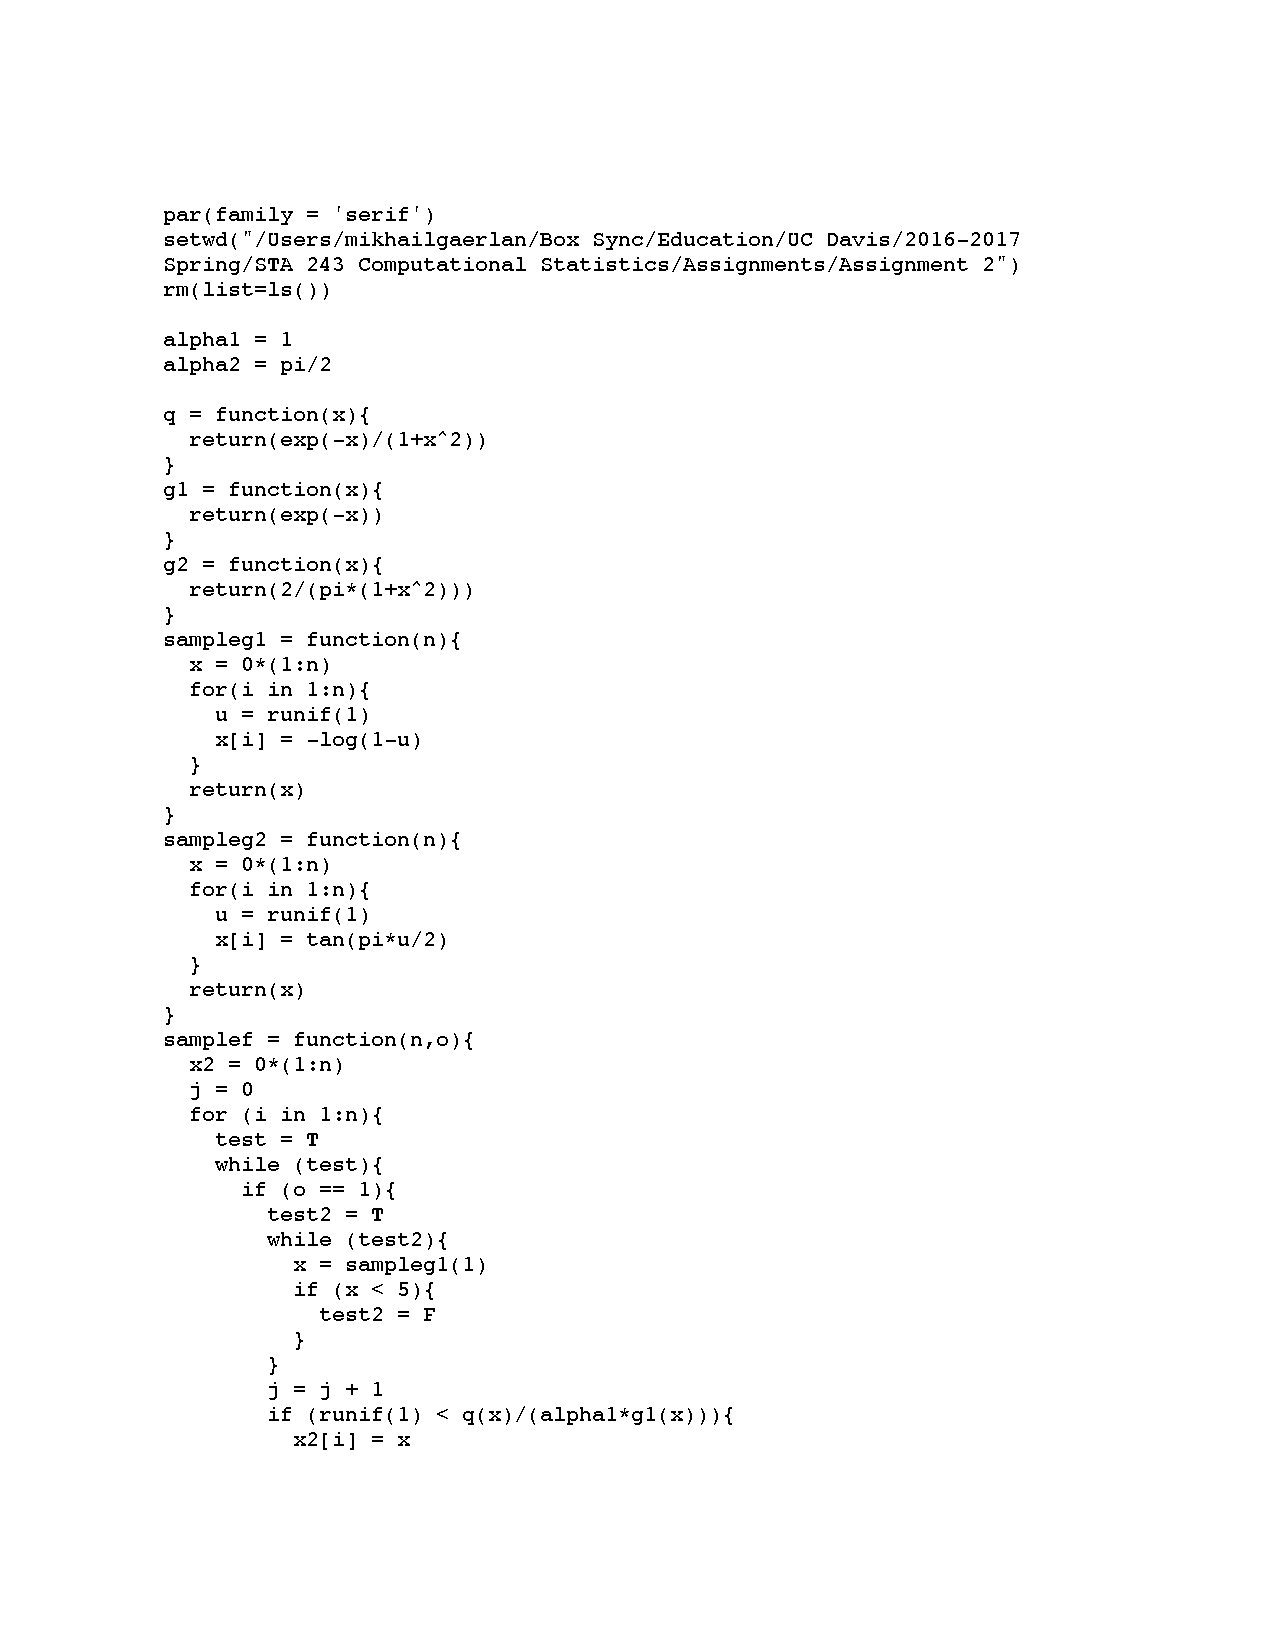
\includepdf[pages={1-2}]{Code/assignment32.pdf}

\end{document}